\section[]{Embedding into Menger Sponge}
\begin{frame}{The Menger Sponge, \cite{menger2002karl}}
\begin{itemize}
    \item Universal - Contains every curve
\end{itemize}
    \begin{figure}
        \centering
        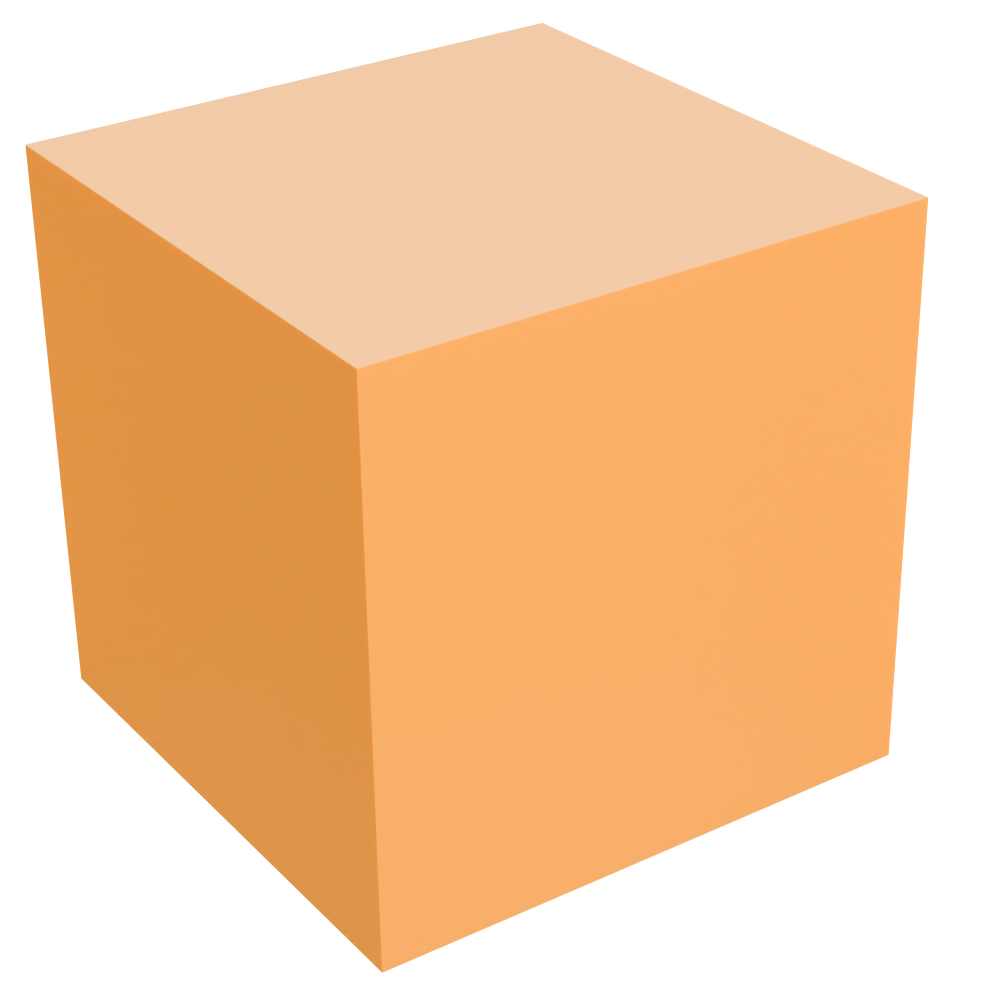
\includegraphics[width=0.25\linewidth]{MichaelImages/Cube.png}
        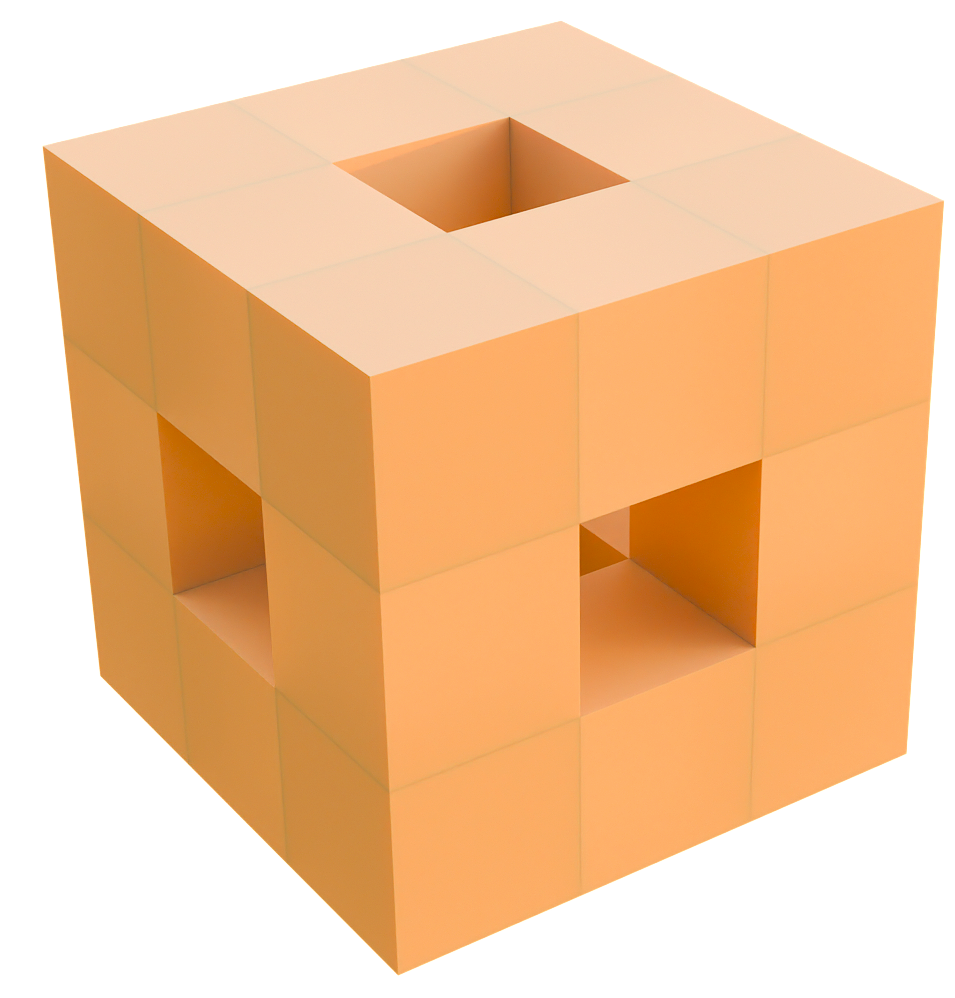
\includegraphics[width=0.25\linewidth]{MichaelImages/FirstIterationCube.png}
         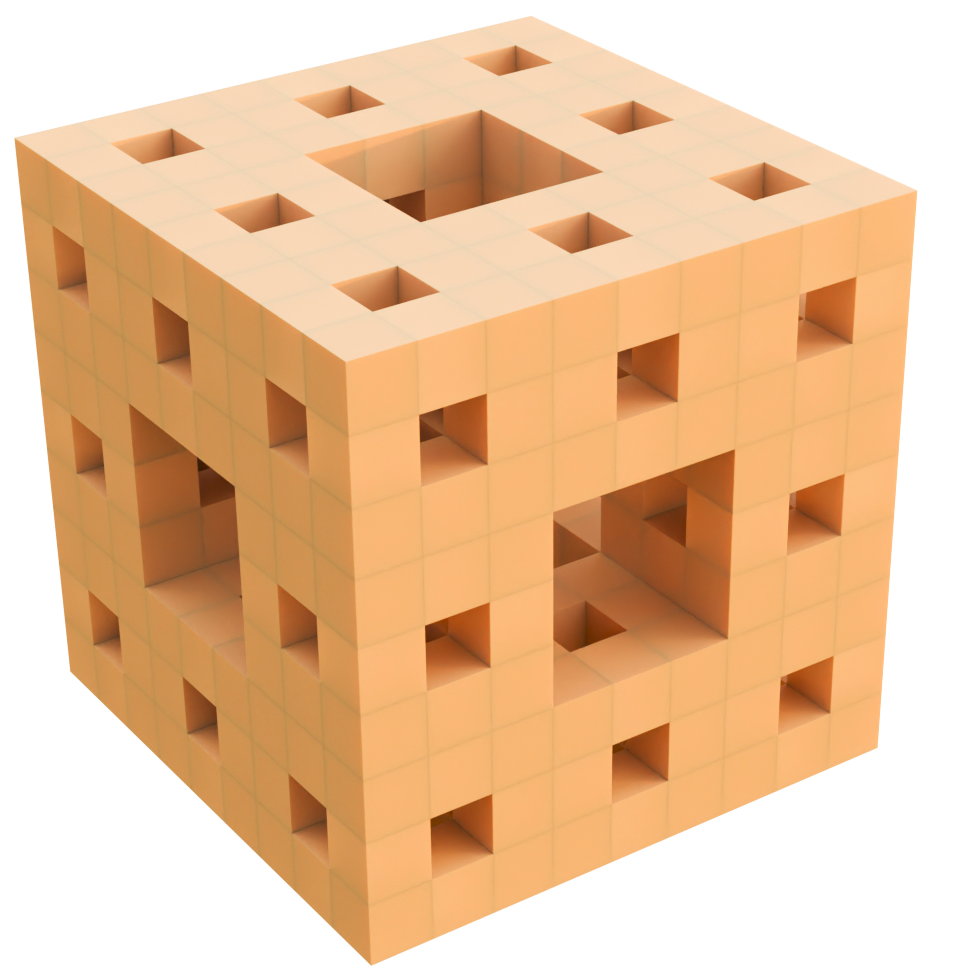
\includegraphics[width=0.25\linewidth]{MichaelImages/SecondIterationCube.png}
        \caption{Michael McGloin (2025)}
        \label{fig:enter-label}
    \end{figure}
\end{frame}

\begin{frame}{Knots Inside the Menger Sponge}
    What is a knot in the Menger Sponge?
    \begin{figure}
        \centering
        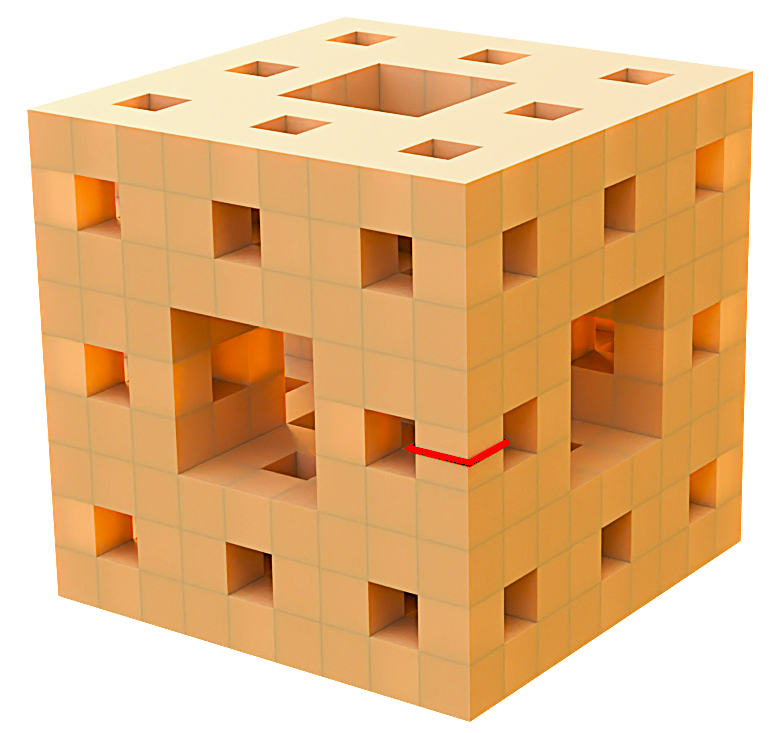
\includegraphics[width=0.35\linewidth]{UnknotTwo.png}
        \caption{The Unknot? - Michael McGloin (2025)}
        \label{fig:enter-label}
    \end{figure}
\end{frame}
\begin{frame}{Not a Knot!}
\begin{figure}
    \centering
    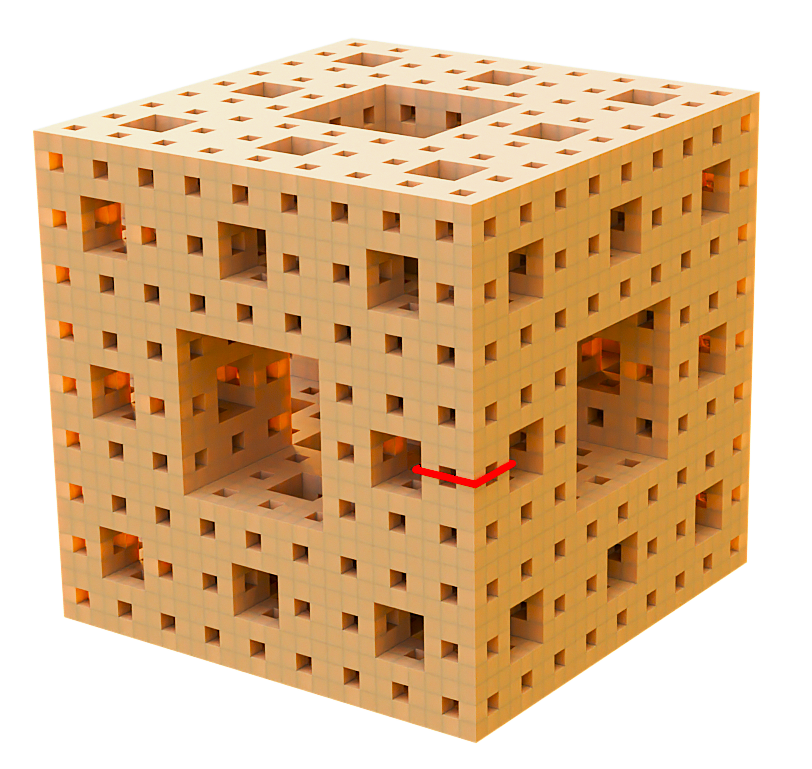
\includegraphics[width=0.49\linewidth]{NotAKnot.png}
    \label{fig:enter-label}
\end{figure}
\end{frame}

\begin{frame}{Knot or Not?}
\begin{itemize}
    \item Does the following knot live on the fractal?

    \begin{figure}
        \centering
        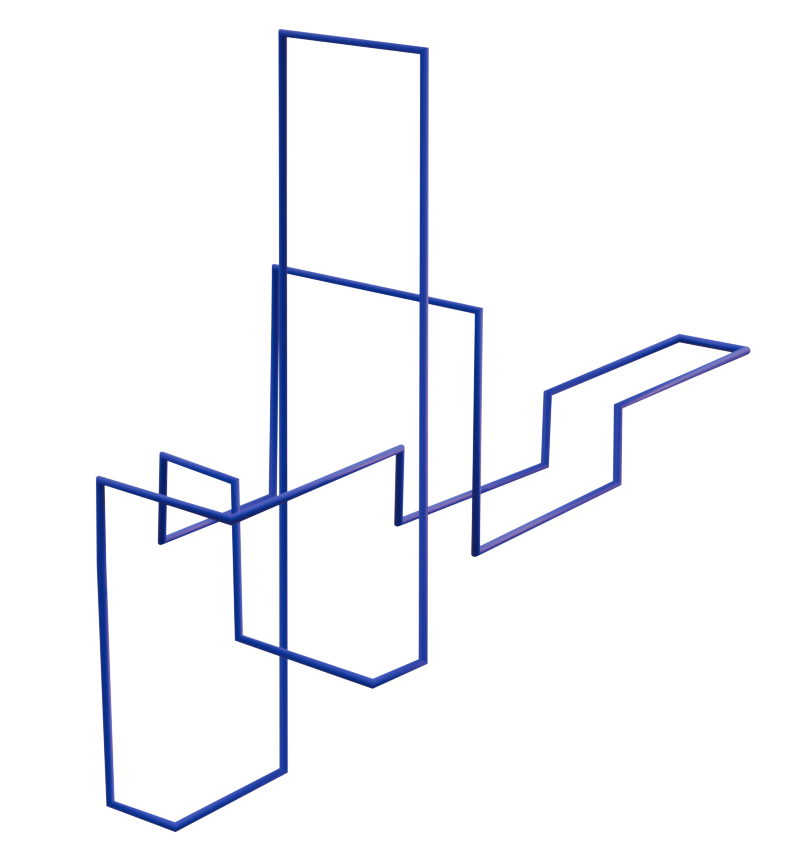
\includegraphics[width=0.25\linewidth]{NoCubeTrefoil.png}
        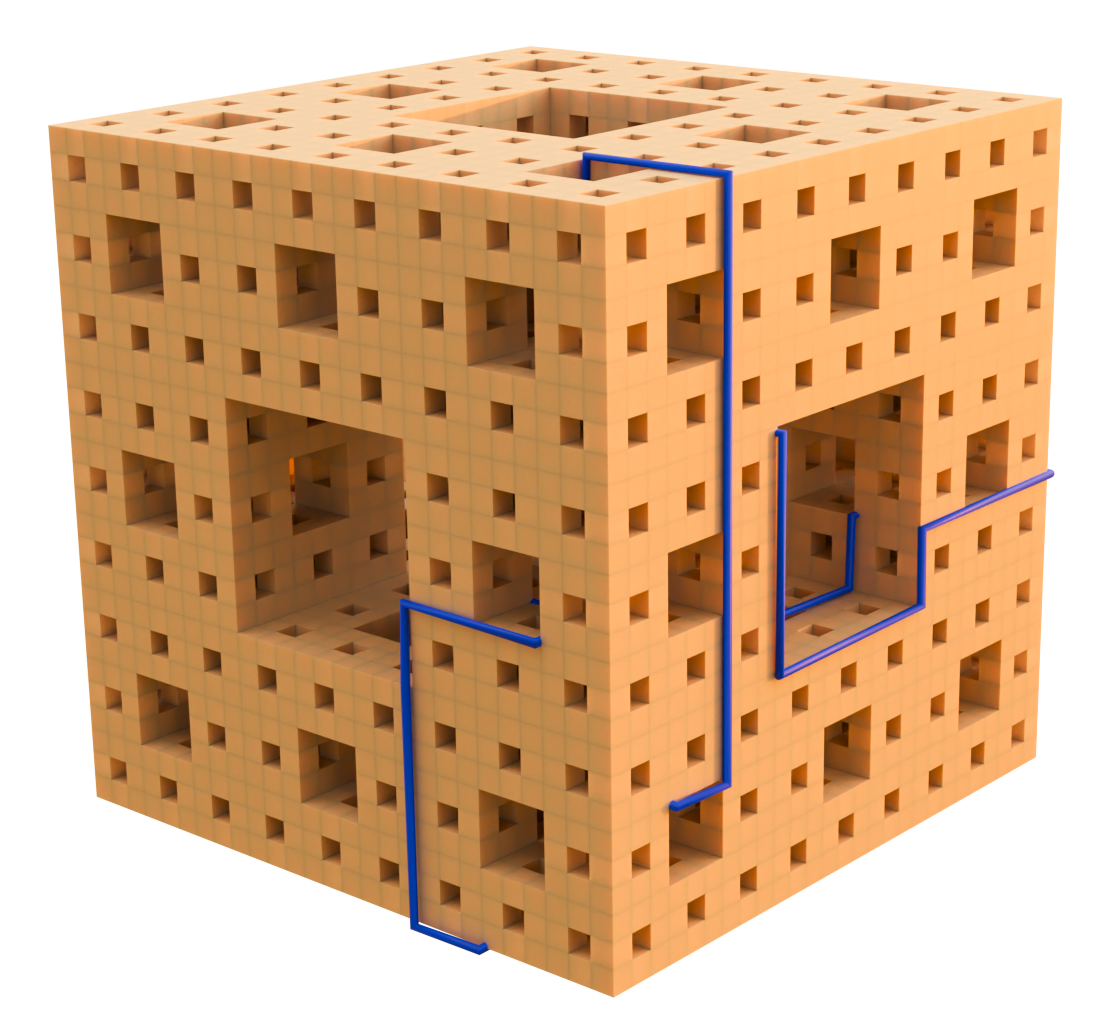
\includegraphics[width=0.3\linewidth]{TreFoilKnot.png}
        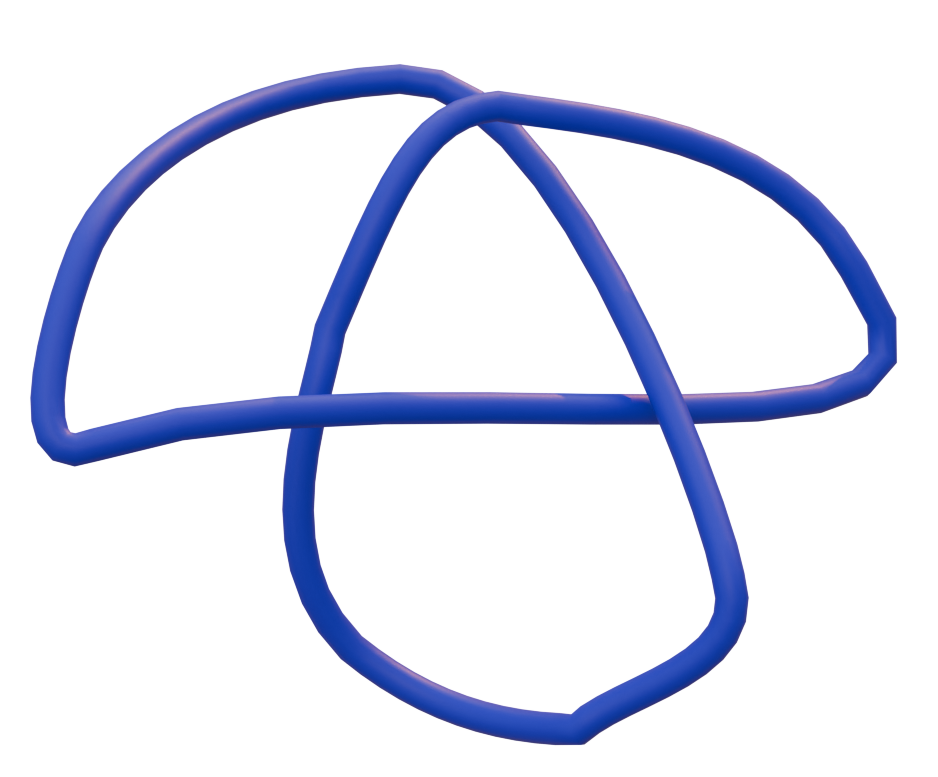
\includegraphics[width=0.3\linewidth]{UnravelledTrefoil.png}
        \caption{Trefoil Knot in Sponge - Michael McGloin (2025)}
        \label{fig:enter-label}
    \end{figure}
    \item What possible knots can we find in this fractal?
\end{itemize}
\end{frame}

\begin{frame}{The Positive Answer}
\begin{itemize}
	\item  This is the question asked by a group of highschoolers.
    \item In 2024 they were able to show that you could find every possible knot embedded in the Menger Sponge!
    \item Published a paper on ArXiv.    
\end{itemize}
 \begin{figure}
     \centering
     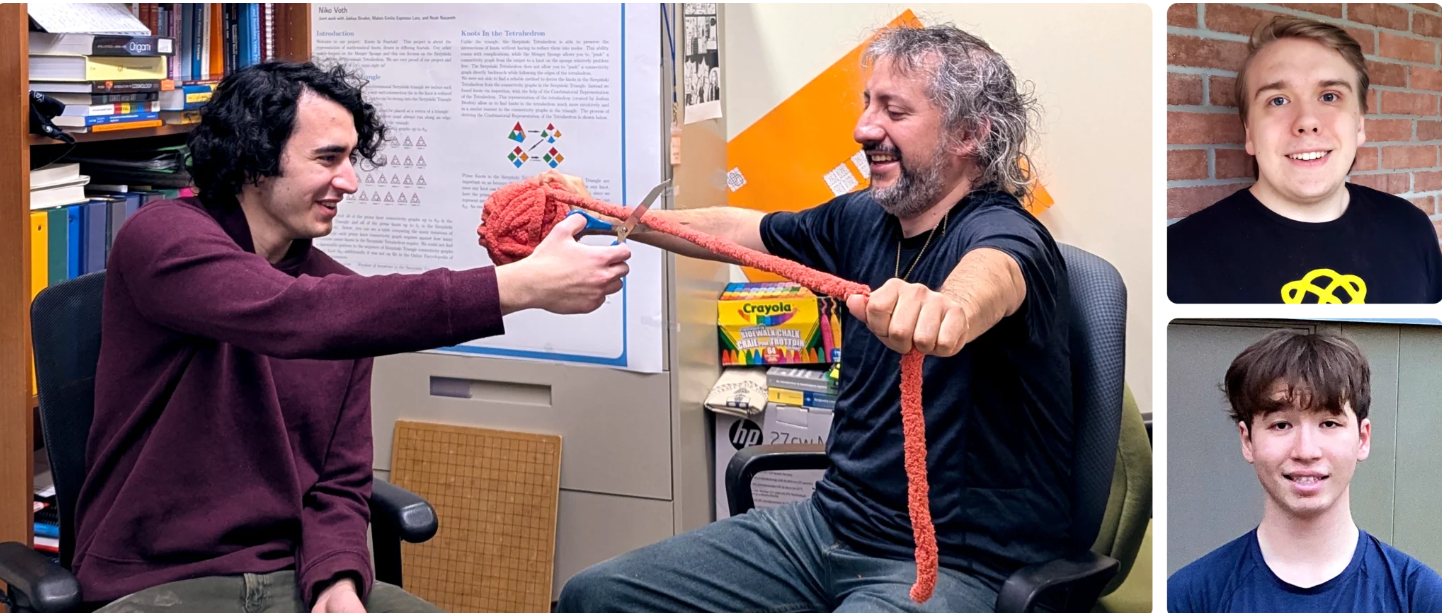
\includegraphics[width=0.5\linewidth]{PhotoOfAuthors.png}
     \caption{Niko Voth (top right), Joshua Broden (bottom right) and Noah Nazareth under the supervision of Malors. \cite{Quanta}}
     \label{fig:enter-label}
 \end{figure}
\end{frame}

\begin{frame}[c]{The Cantor Set}
\begin{itemize}
    \item Split the interval $[0,1]$ into thirds and remove the middle third
    \item Repeat on each remaining interval
\end{itemize}
\begin{figure}
    \centering
    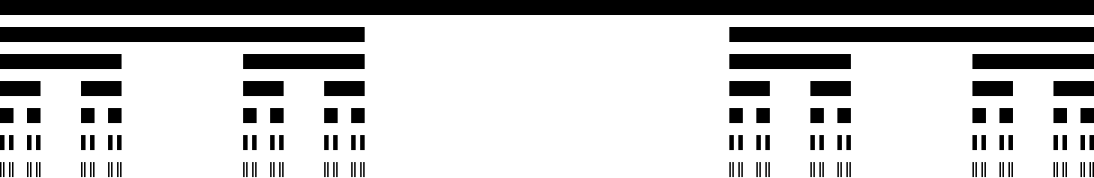
\includegraphics[width=0.7\linewidth]{Cantor_set_in_seven_iterations.svg.png}
    \caption{Cantor Set - \cite{cantor}}
    \label{fig:enter-label}
\end{figure}
\end{frame}

\begin{frame}{Cantor Dust}
Cantor dust is a 2 dimensional fractal and is the cartesian product of 2 cantor sets
 \begin{figure}
     \centering
     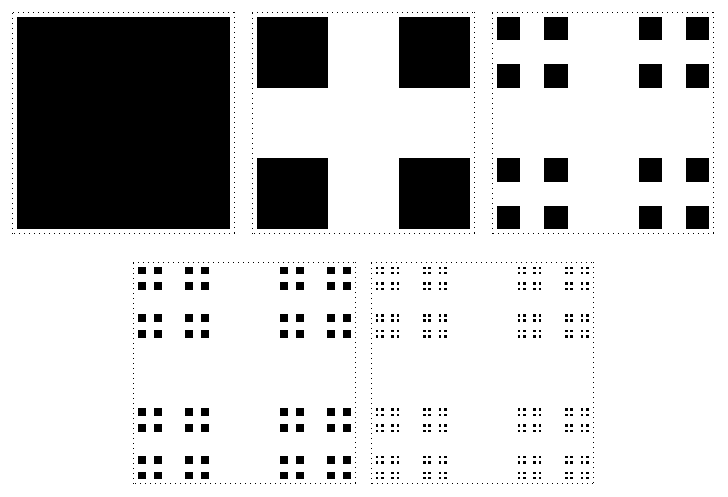
\includegraphics[width=0.5\linewidth]{cantordust.png}
     \caption{\cite{Dickau_Cantor_Dust}}
     \label{fig:enter-label}
 \end{figure}
\end{frame}

\begin{frame}{Relation With Sierpienski Carpet}
 \begin{lemma}
     $(x,y)$ lies on the Sierpinski carpet if and only if $x$ and $y$ share no digit $1$ in their ternary expansion.
 \end{lemma}
\begin{figure}
    \centering
    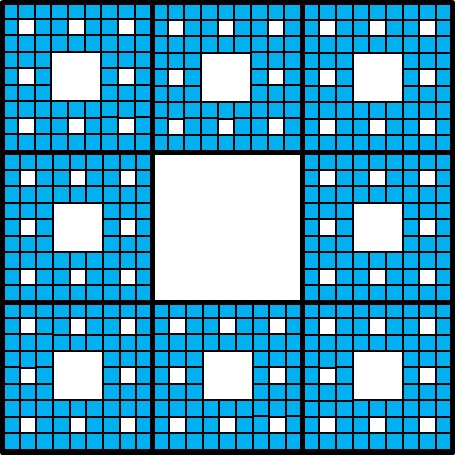
\includegraphics[width=0.2\linewidth]{Carpet.jpg}
    \caption{Sierpinski Carpet, \cite{sierpinski2016}}
    \label{fig:enter-label}
\end{figure}
\end{frame}

\begin{frame}{Which Points Lie on the Menger Sponge?}
\begin{lemma}
    Let $ (x, y)$ be a Cantor Dust point, then $(x,y,z) \in M$ for all $0 \leq z \leq 1$.
\end{lemma}

\begin{proof}
Consider the first 2 stages where regions not in black have a hole behind them. 
    \begin{figure}
        \centering
        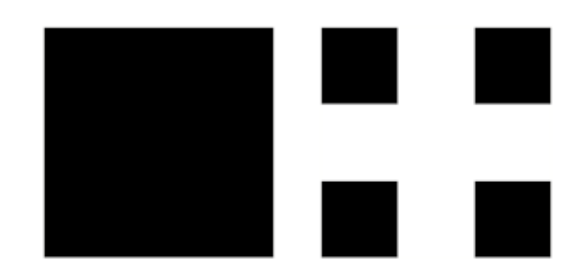
\includegraphics[width=0.22\linewidth]{ProofOfPointsOnSponge.png}
        \caption{Stage 0 and Stage 1 \cite{broden2024knotsinsidefractals}}
        \label{fig:enter-label}
    \end{figure}
\end{proof}
\end{frame}

\begin{frame}[c]{Cantor Dust!}
	 \begin{figure}
		\centering
		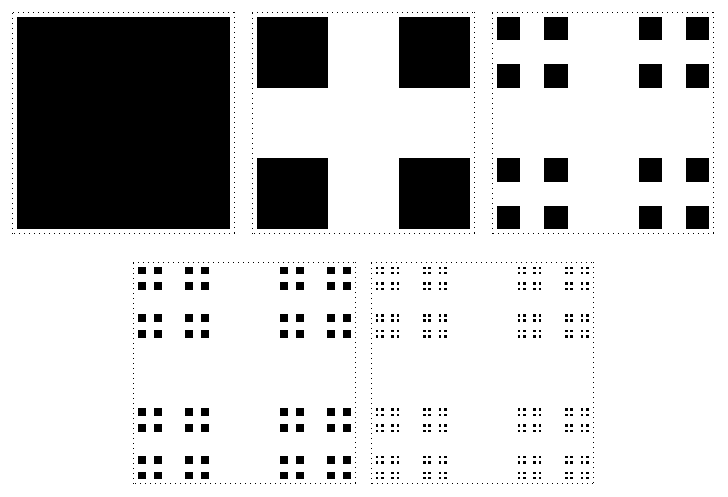
\includegraphics[width=0.5\linewidth]{cantordust.png}
		\caption{\cite{Dickau_Cantor_Dust}}
		\label{fig:enter-label}
	\end{figure}
\end{frame}

\begin{frame}{Arc Presentation and Arc Index}
An arc presentation of a knot K is an embedding of K in finitely many pages of the open-book decomposition so that each of these pages meets K in a single simple arc
\begin{figure}
    \centering
    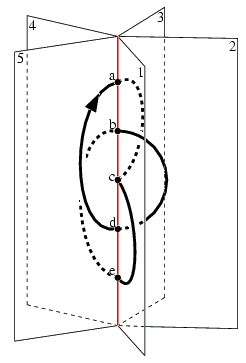
\includegraphics[width=0.2\linewidth]{MichaelImages/arc_index_fig1.png} $K = \{3,5\}, \{2,4\}, \{1,3\}, \{2,5\}, \{1,4\} $
    \caption{Arc Presentation Trefoil, \cite{inproceedings}}
    \label{fig:enter-label}
\end{figure}
\end{frame}

\begin{frame}{Arc Presentation and Arc Index}
\vspace{20px}
\begin{definition}
    The minimum number of pages required to represent a knot is called its arc index
\end{definition}

\begin{example}
    The arc index of a $(p,q)$ torus knot is $p+q$. This was shown using techniques from contact geometry. (\cite{etnyre2000knotscontactgeometry})
\end{example}
\end{frame}

\begin{frame}[c]{Knots in The Menger Sponge}
We now give the proof that every knot can be found in a finite iteration of the merger sponge.
\begin{itemize}
    \item Let $K = \{a_1, b_1\}, \dots, \{a_n, b_n\}$ be its arc presentation.
    \item Take $n$ endpoints, $p_1, \dots p_n $ of Cantor Set.
    \item We now re-write $K = \{p_{a_1}, p_{b_1}\} \dots \{p_{a_n}, p_{b_n}\}$
\end{itemize}
\end{frame}

\begin{frame}[c]{Knots in The Menger Sponge}
\begin{itemize}
    \item We notice if $x_0 \in C$ then vertical line through $x_0 $ on sponge.
    \item Same with vertical lines for $y_0$
    \item Can draw our knot diagram on the face!
\end{itemize}

\begin{figure}
    \centering
    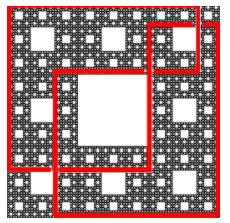
\includegraphics[width=0.2\linewidth]{KnotOnFace.png}
    \caption{\cite{broden2024knotsinsidefractals}}
    \label{fig:enter-label}
\end{figure}
\end{frame}

\begin{frame}[c]{Push Through the Sponge!}
The last big idea is to push the knot through the sponge
\begin{itemize}
    \item Vertical lines on front face.
    \item Horizontal Lines on back face.
    \item We connect them through the sponge.
    \item The knot is our original knot as the projection onto the front face recovers our knot diagram.
\end{itemize}
\end{frame}

\begin{frame}[c]{Knot Game}
	\begin{center}
		Before we start the proof we will play a quick game!
		The goal is to guess the correct knot inside the sponge.
	\end{center}
	
	
\end{frame}